\documentclass{article}
\usepackage{times}
\usepackage{listings}
\usepackage{graphicx}
\usepackage{pdfpages}
\usepackage{geometry}
\geometry{a4paper, margin=1in}

\title{CSE 4102 Lab Project Report}
\author{Tonmoy}
\date{\today}

\begin{document}

% Replace 'cover.pdf' with the actual filename of the PDF you want to include
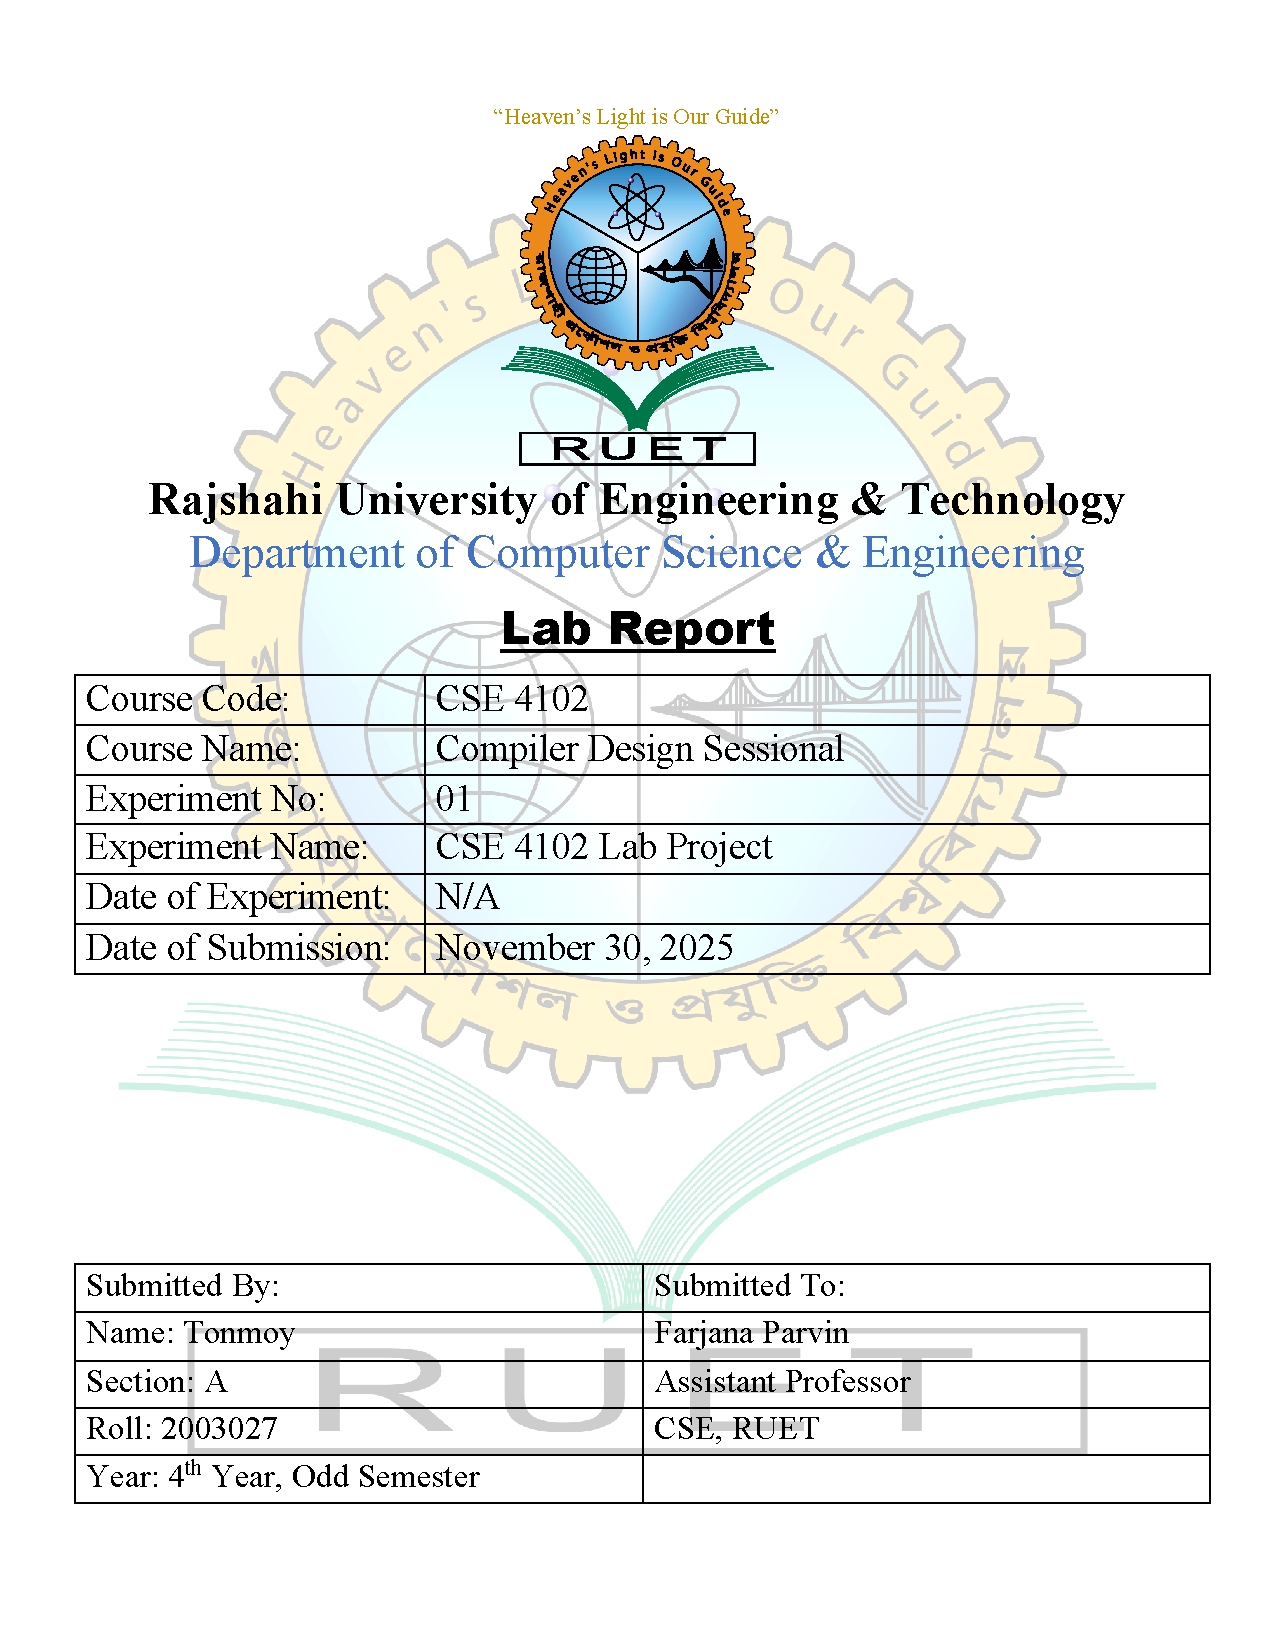
\includepdf[pages=-]{cover.pdf}

\maketitle

\section{Introduction}
This report documents the design and implementation of a compiler for a custom programming language. The project involves the development of a lexical analyzer using Flex and a parser using Bison. The compiler translates the source code into an intermediate representation and subsequently generates x86 assembly code. The report details the various phases of compilation, including lexical analysis, syntax analysis, intermediate code generation, and final assembly code generation, demonstrating the complete translation process from high-level source code to machine-executable instructions.

\section{Input Code}
The following is the input source code provided in \texttt{input.txt}. This code is written in a custom programming language that supports variable declarations, assignments, arithmetic operations, and printing. The syntax includes keywords like \texttt{FUNC}, \texttt{start}, \texttt{end}, \texttt{mone\_kori} (declare), \texttt{jog} (add), and \texttt{print\_kori} (print).

\begin{lstlisting}[frame=single]
FUNC main () 
start
       mone_kori a <-- integer
       mone_kori b <-- integer
       a equal 12
       b equal 13 jog a
       print_kori b
end
\end{lstlisting}

\section{Output Analysis}

\subsection{Lexical Analysis}
This section demonstrates the output of the lexical analyzer (Lex). The lexer scans the source code character by character and groups them into meaningful tokens such as keywords, identifiers, operators, and constants. Additionally, during this phase, identifiers are inserted into the symbol table with their respective types and assigned memory addresses.

\begin{lstlisting}[frame=single, breaklines=true]
Token: FUNC
Token: ID, Value: main
Token: LPAREN
Token: RPAREN
Token: START_BLOCK
Token: MONE_KORI
Token: ID, Value: a
Token: DECLARATION
Token: INTEGER
In line no 3, Inserting a with type INT_TYPE in symbol table at address 0.
Token: MONE_KORI
Token: ID, Value: b
Token: DECLARATION
Token: INTEGER
In line no 4, Inserting b with type INT_TYPE in symbol table at address 1.
Token: ID, Value: a
Token: EQUAL
Token: ICONST, Value: 12
Token: ID, Value: b
Token: EQUAL
Token: ICONST, Value: 13
Token: JOG
Token: ID, Value: a
Token: PRINT_KORI
Token: ID, Value: b
Token: END_BLOCK
\end{lstlisting}

\begin{figure}[h]
    \centering
    % Replace 'lexical_output.png' with your actual screenshot file
    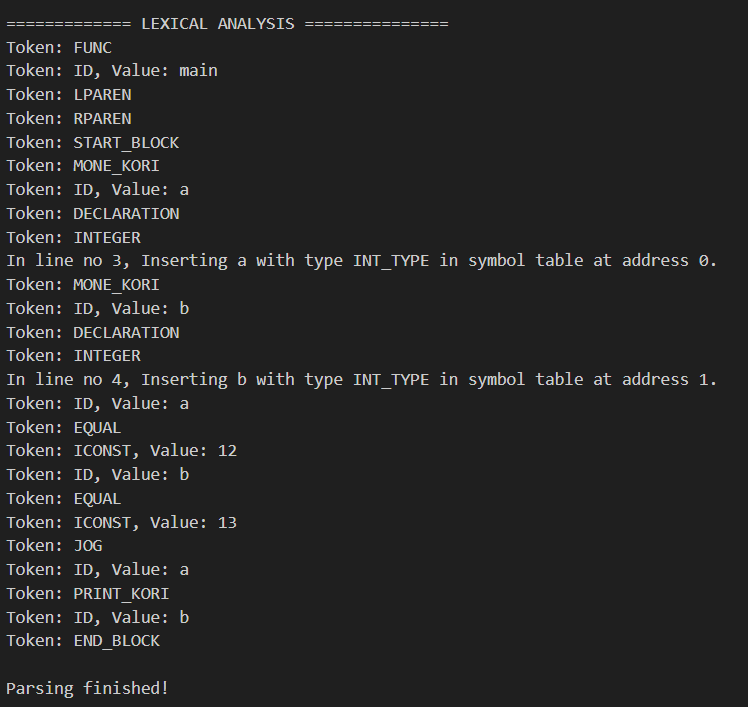
\includegraphics[width=\textwidth]{lexical_output.png}
    \caption{Lexical Analysis Output}
\end{figure}

\subsection{Syntax Analysis (Parse Tree)}
This section illustrates the syntax analysis phase performed by the parser (Bison). It displays the sequence of grammar rules (reductions) applied to the stream of tokens to verify the grammatical structure of the program. The output represents a bottom-up traversal of the parse tree, showing how lower-level constructs (like expressions and statements) are combined to form higher-level constructs (like functions and programs).

\begin{lstlisting}[frame=single, breaklines=true]
declaration -> MONE_KORI ID DECLARATION INTEGER
statement -> declaration
statements -> statement
declaration -> MONE_KORI ID DECLARATION INTEGER
statement -> declaration
statements -> statements statement
exp -> ICONST
assignment -> ID EQUAL exp
statement -> assignment
statements -> statements statement
exp -> ICONST
exp -> ID
exp -> exp JOG exp
assignment -> ID EQUAL exp
statement -> assignment
statements -> statements statement
print_statement -> PRINT_KORI ID
statement -> print_statement
statements -> statements statement
function -> FUNC ID LPAREN RPAREN START_BLOCK statements END_BLOCK
program -> function
\end{lstlisting}

\begin{figure}[h]
    \centering
    % Replace 'syntax_output.png' with your actual screenshot file
    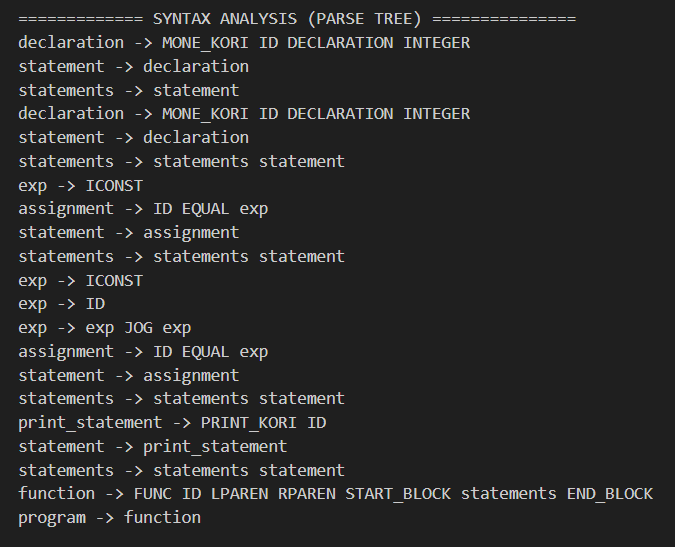
\includegraphics[width=\textwidth]{syntax_output.png}
    \caption{Syntax Analysis Output}
\end{figure}

\subsection{Intermediate Code}
This section presents the generated intermediate code, which serves as an abstraction between the high-level source code and the low-level machine code. The intermediate representation used here is a stack-based instruction set. Instructions such as \texttt{ld\_int} (load integer), \texttt{ld\_var} (load variable), \texttt{store}, and \texttt{add} operate on a virtual stack to perform the computations defined in the source program.

\begin{lstlisting}[frame=single]
  0: start              -1
  1: ld_int             12
  2: store               0
  3: ld_int             13
  4: ld_var              0
  5: add                -1
  6: store               1
  7: print_int_value     1
  8: halt               -1
\end{lstlisting}

\begin{figure}[h]
    \centering
    % Replace 'intermediate_output.png' with your actual screenshot file
    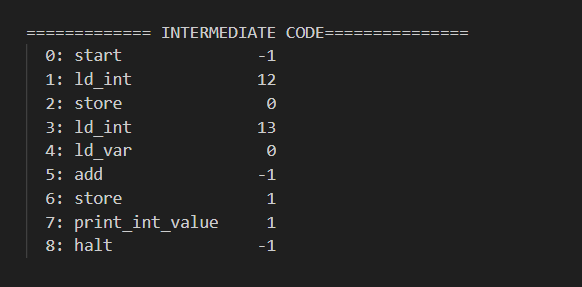
\includegraphics[width=\textwidth]{intermediate_output.png}
    \caption{Intermediate Code Output}
\end{figure}

\subsection{ASM Code}
This section displays the final x86 assembly code generated from the intermediate representation. The code is targeted for the MASM (Microsoft Macro Assembler) environment. It includes the necessary headers, stack setup, and data segment definitions. The instructions translate the stack-based intermediate operations into register-based x86 instructions (e.g., \texttt{MOV}, \texttt{ADD}, \texttt{PUSH}, \texttt{POP}) to be executed on the processor.

\begin{lstlisting}[frame=single, language={[x86masm]Assembler}, breaklines=true]
;start -1
.686
.model flat, c
include C:\masm32\include\msvcrt.inc
includelib C:\masm32\lib\msvcrt.lib

.stack 100h
printf PROTO arg1:Ptr Byte, printlist:VARARG
scanf PROTO arg2:Ptr Byte, inputlist:VARARG

.data
output_integer_msg_format byte "%d", 0Ah, 0
output_string_msg_format byte "%s", 0Ah, 0
input_integer_format byte "%d",0

number sdword ?

.code

main proc
	push ebp
	mov ebp, esp
	sub ebp, 100
	mov ebx, ebp
	add ebx, 4

;ld_int 12
	mov eax, 12
	mov dword ptr [ebx], eax
	add ebx, 4


;store 0
	mov dword ptr [ebp-0], eax

;ld_int 13
	mov eax, 13
	mov dword ptr [ebx], eax
	add ebx, 4


;ld_var 0
	mov eax, [ebp-0]
	mov dword ptr [ebx], eax
	add ebx, 4


;add -1
	sub ebx, 4
	mov eax, [ebx]
	sub ebx, 4
	mov edx, [ebx]
	add eax, edx
	mov dword ptr [ebx], eax
	add ebx, 4


;store 1
	mov dword ptr [ebp-4], eax

;print_int_value 1
	push eax
	push ebx
	push ecx
	push edx
	push [ebp-4]
	push [ebp-0]
	push [ebp+4]
	push [ebp+8]
	push ebp
	mov eax, [ebp-4]
	INVOKE printf, ADDR output_integer_msg_format, eax
	pop ebp
	pop [ebp+8]
	pop [ebp+4]
	pop [ebp-0]
	pop [ebp-4]
	pop edx
	pop ecx
	pop ebx
	pop eax

;halt -1
	add ebp, 100
	mov esp, ebp
	pop ebp
	ret
main endp
end
\end{lstlisting}

\begin{figure}[h]
    \centering
    % Replace 'asm_output.png' with your actual screenshot file
    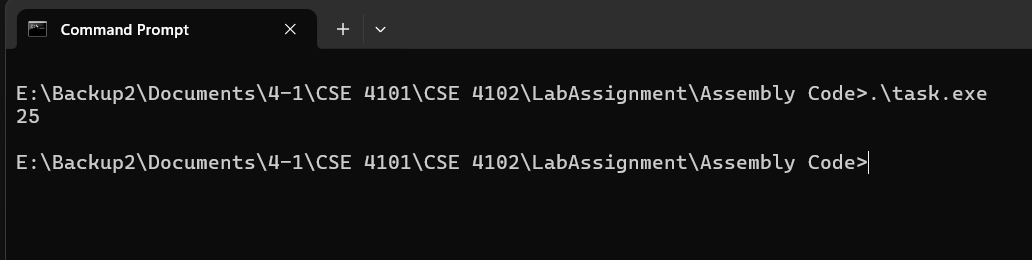
\includegraphics[width=\textwidth]{asm_output.png}
    \caption{ASM Code Output}
\end{figure}

\section{Conclusion}
In conclusion, this project successfully demonstrates the construction of a functional compiler for a subset of a custom programming language. By integrating Flex for lexical analysis and Bison for syntax analysis, the system effectively parses source code and generates valid intermediate and assembly code. The step-by-step analysis of the output confirms the correctness of the symbol table management, parse tree construction, and code generation logic. This assignment provided valuable practical experience in understanding the internal mechanisms of compiler design and the translation of high-level constructs into low-level machine instructions.

\end{document}
